% ============================================================================
% Seccion 4 — Proceso ETL para la base de datos (punto 4 del enunciado)
% ============================================================================
\section{Proceso ETL para la base de datos}

\subsection{Arquitectura de tablas definida por el grupo}
Se eligi\'o un \textbf{modelo estrella} porque el dataset ya viene en forma de cubo: la tabla de
hechos guarda la medida (\texttt{cantidad}) y las claves de las dimensiones, y cada dimensi\'on
guarda los atributos con los que se agrupa o filtra. Las claves primarias son naturales
(el propio valor del dataset), lo que hace el ETL verificable: cualquier fila del CSV se puede
seguir hasta la tabla de hechos.

\begin{figure}[H]
\centering
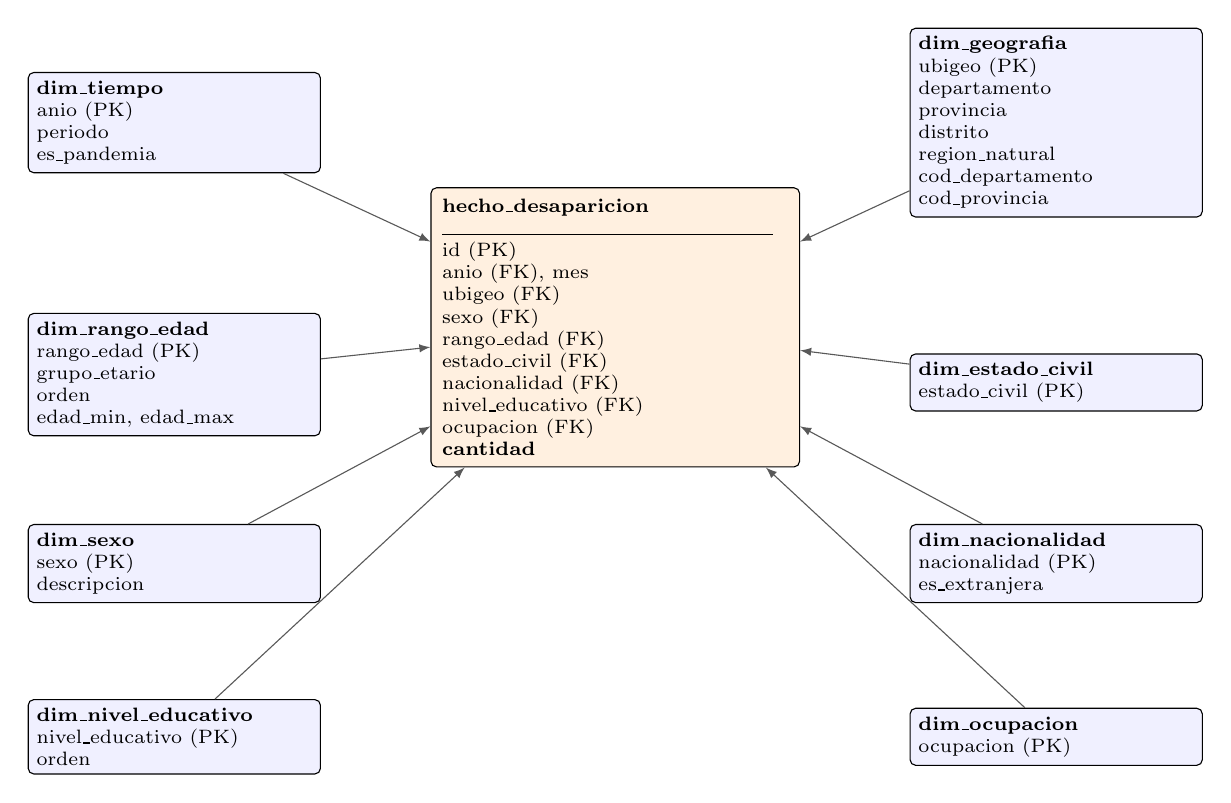
\begin{tikzpicture}[
  every node/.style={font=\scriptsize},
  dim/.style={draw, fill=blue!6, rounded corners=2pt, inner sep=3pt, align=left, text width=3.5cm},
  fac/.style={draw, fill=orange!12, rounded corners=2pt, inner sep=4pt, align=left, text width=4.4cm},
  link/.style={-latex, gray!70!black}
]
\node[fac] (hecho) at (0,0) {
  \textbf{hecho\_desaparicion}\\
  \rule{4.2cm}{0.2pt}\\
  id (PK)\\
  anio (FK), mes\\
  ubigeo (FK)\\
  sexo (FK)\\
  rango\_edad (FK)\\
  estado\_civil (FK)\\
  nacionalidad (FK)\\
  nivel\_educativo (FK)\\
  ocupacion (FK)\\
  \textbf{cantidad}
};
\node[dim] (tiempo) at (-5.6, 2.6) {\textbf{dim\_tiempo}\\ anio (PK)\\ periodo\\ es\_pandemia};
\node[dim] (geo)    at (5.6, 2.6)  {\textbf{dim\_geografia}\\ ubigeo (PK)\\ departamento\\ provincia\\ distrito\\ region\_natural\\ cod\_departamento\\ cod\_provincia};
\node[dim] (edad)   at (-5.6, -0.6) {\textbf{dim\_rango\_edad}\\ rango\_edad (PK)\\ grupo\_etario\\ orden\\ edad\_min, edad\_max};
\node[dim] (sexo)   at (-5.6, -3.0) {\textbf{dim\_sexo}\\ sexo (PK)\\ descripcion};
\node[dim] (civil)  at (5.6, -0.7) {\textbf{dim\_estado\_civil}\\ estado\_civil (PK)};
\node[dim] (nacion) at (5.6, -3.0) {\textbf{dim\_nacionalidad}\\ nacionalidad (PK)\\ es\_extranjera};
\node[dim] (nivel)  at (-5.6, -5.2) {\textbf{dim\_nivel\_educativo}\\ nivel\_educativo (PK)\\ orden};
\node[dim] (ocup)   at (5.6, -5.2) {\textbf{dim\_ocupacion}\\ ocupacion (PK)};
\draw[link] (tiempo) -- (hecho);
\draw[link] (geo) -- (hecho);
\draw[link] (edad) -- (hecho);
\draw[link] (sexo) -- (hecho);
\draw[link] (civil) -- (hecho);
\draw[link] (nacion) -- (hecho);
\draw[link] (nivel) -- (hecho);
\draw[link] (ocup) -- (hecho);
\end{tikzpicture}
\caption{Diagrama entidad-relaci\'on del modelo estrella implementado en PostgreSQL 16.
\texttt{hecho\_desaparicion} referencia las ocho dimensiones; \texttt{dim\_geografia} tiene una
fila por ubigeo (1,506).}
\label{fig:er}
\end{figure}

Adem\'as del modelo final se cre\'o una tabla de \textbf{staging} (\texttt{stg\_desaparicion})
con las 13 columnas tal como llegan del CSV. Esta tabla materializa el paso de extracci\'on y
permite reejecutar la transformaci\'on sin volver a descargar el archivo.

\subsection{Extracci\'on}
El dataset se descarga del portal de la PNDA como un \'unico CSV de 8.1 MB. La extracci\'on se
hace con \texttt{COPY} de PostgreSQL, que es la v\'ia m\'as r\'apida para archivos locales y no
requiere herramientas externas:

\begin{lstlisting}[style=sql]
COPY stg_desaparicion (anio, mes, ubigeo_hecho, dpto_hecho, prov_hecho, dist_hecho,
                       sexo, rango_edad, est_civil, nacionalidad, nivel_educativo,
                       ocupacion, cantidad)
FROM '/home/arbues/macrodatos/PC3/data/denuncias_desaparicion_2019_2024.csv'
WITH (FORMAT csv, HEADER true, DELIMITER ',', ENCODING 'UTF8', NULL '');
\end{lstlisting}

\subsection{Transformaci\'on}
Sobre la tabla de staging se aplican seis reglas, todas verificables en \texttt{sql/02\_etl.sql}:

\begin{enumerate}
  \item \textbf{Categ\'oricas vac\'ias a \texttt{NO ESPECIFICA}}: se aplica a \texttt{sexo},
        \texttt{rango\_edad}, \texttt{est\_civil}, \texttt{nacionalidad},
        \texttt{nivel\_educativo} y \texttt{ocupacion}. No se imputa ning\'un valor del dataset.
  \item \textbf{Ubigeo}: se normaliza a 6 caracteres con \texttt{LPAD} y se agrupa por ubigeo
        tomando un solo nombre por distrito, porque el c\'odigo \texttt{150121} aparece con dos
        graf\'ias (PUEBLO LIBRE y MAGDALENA VIEJA). Sin este paso, cada join con la dimensi\'on
        geogr\'afica duplicar\'ia 82 personas.
  \item \textbf{Regi\'on natural}: se deriva del departamento con una regla \texttt{CASE}
        (12 departamentos de costa, 10 de sierra, 4 de selva).
  \item \textbf{Periodo pand\'emico}: 2019 = pre-pandemia, 2020--2021 = pandemia,
        2022--2024 = post-pandemia.
  \item \textbf{Grupo etario}: los seis rangos del dataset se agrupan en primera infancia, ni\~nez,
        adolescente, adulto joven, adulto y adulto mayor, con un orden num\'erico para ordenar
        resultados sin depender del texto.
  \item \textbf{Filtro de calidad}: solo se cargan hechos con \texttt{cantidad} positiva y no
        nula (en la pr\'actica, el 100\,\% de las filas).
\end{enumerate}

\subsection{Llenado}
El orden de carga respeta las dependencias: primero las ocho dimensiones y despu\'es la tabla de
hechos, todo dentro de una sola transacci\'on para que el ETL sea at\'omico. Las dimensiones se
pueblan con \texttt{INSERT \dots SELECT DISTINCT} sobre el staging, de modo que el cat\'alogo
geogr\'afico (1,506 ubigeos) y los cat\'alogos de nacionalidad (57 valores) y ocupaci\'on (289
valores) se generan del propio dataset.

\begin{lstlisting}[style=sql]
BEGIN;
TRUNCATE stg_desaparicion;
COPY stg_desaparicion (...) FROM :'ruta_csv' WITH (FORMAT csv, HEADER true, ...);
INSERT INTO dim_tiempo ...;
INSERT INTO dim_geografia (...) SELECT DISTINCT ... FROM stg_desaparicion WHERE ubigeo <> '';
INSERT INTO dim_rango_edad ...; INSERT INTO dim_sexo ...;
INSERT INTO dim_nacionalidad (...) SELECT DISTINCT ... ON CONFLICT DO NOTHING;
INSERT INTO dim_ocupacion (...)    SELECT DISTINCT ... ON CONFLICT DO NOTHING;
INSERT INTO hecho_desaparicion (...)
SELECT ... FROM stg_desaparicion WHERE cantidad > 0;
COMMIT;
\end{lstlisting}

\subsection{Verificaci\'on del ETL}
El script cierra con tres controles que se muestran en las capturas de la base de datos
funcionando (\texttt{evidencias/pg-*.png}):
\begin{itemize}
  \item conteo de filas por tabla: \texttt{hecho\_desaparicion} = 93,831,
        \texttt{dim\_geografia} = 1,506, \texttt{dim\_nacionalidad} = 57,
        \texttt{dim\_ocupacion} = 289;
  \item control de cuadre: \texttt{SUM(cantidad)} = 121,427, id\'entico al calculado en Spark;
  \item consulta de comprobaci\'on sobre la vista \texttt{v\_desaparicion} (top 10 de
        departamentos por personas), que devuelve exactamente el mismo orden que la consulta
        5a.1 ejecutada en Spark.
\end{itemize}

\IfFileExists{../evidencias/pg-version.png}{
\begin{figure}[H]
\centering
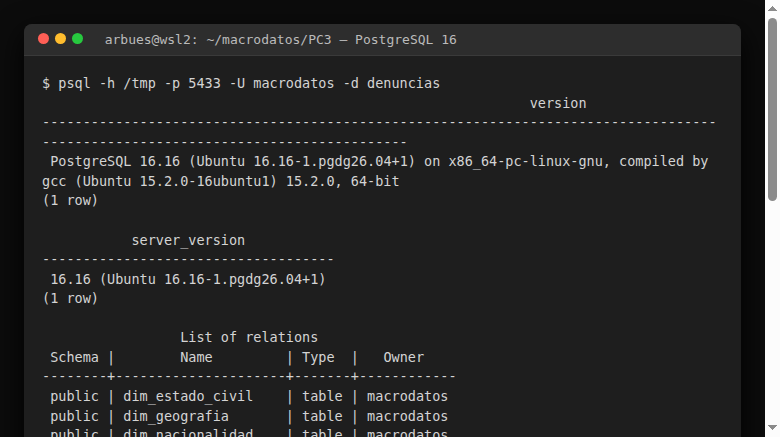
\includegraphics[width=0.9\textwidth]{../evidencias/pg-version.png}
\caption{Servidor PostgreSQL 16 en funcionamiento y verificaci\'on de la versi\'on.}
\end{figure}}{}

\IfFileExists{../evidencias/pg-conteos.png}{
\begin{figure}[H]
\centering
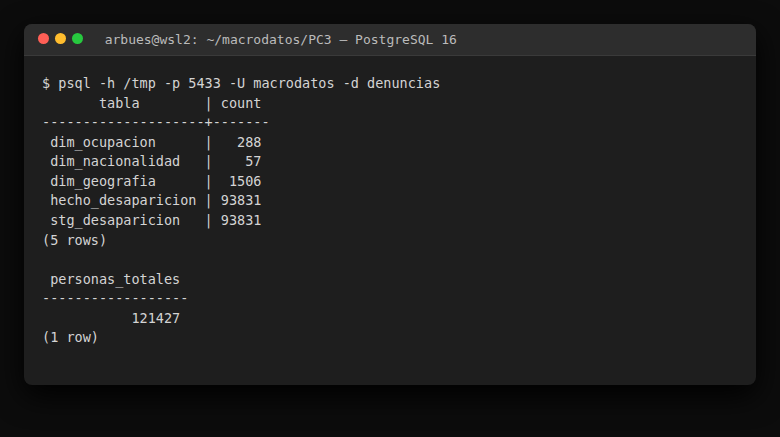
\includegraphics[width=0.9\textwidth]{../evidencias/pg-conteos.png}
\caption{Conteos por tabla y control de cuadre del ETL (121,427 personas).}
\end{figure}}{}

\IfFileExists{../evidencias/pg-consulta.png}{
\begin{figure}[H]
\centering
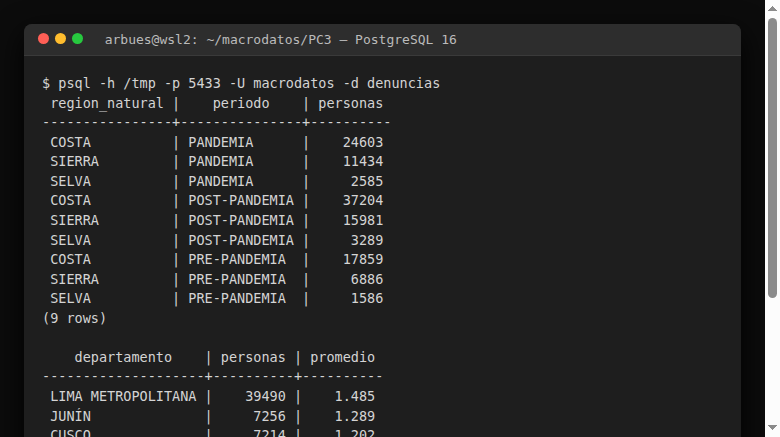
\includegraphics[width=0.9\textwidth]{../evidencias/pg-consulta.png}
\caption{Consulta de comprobaci\'on sobre la vista \texttt{v\_desaparicion}.}
\end{figure}}{}
